\paragraph*{}
In the previous section we described how the neural network that provides us with the initial performance estimates works. However, if that was all our agent did, an error in its output would mean that we're stuck with a sub-optimal agent for all sessions in a certain domain. % TODO: better way to say it
Luckily, we can observe the result of each session \textendash \ the utility we gained  \textendash \ and we can judge if our estimates are correct or if they need adjusting.

\paragraph*{}
To do that, just like \cite{meta_agent_paper}, we model the competition as a Multi-Armed Bandit (MAB) setting, as defined in \cite{MAB_Lai_Robbins_1985} and \cite{MAB_paper_2002}: we have several agents in our arsenal (the \emph{arms}) and in each negotiation session (a MAB \emph{round}) we pick one and gain some utility (\emph{reward}). Such settings are well studied in the Reinforcement Learning (RL) literature and many algorithmic approaches exist to solving them. % TODO: language

\paragraph*{}
Of those algorithms we chose the Upper Confidence Bound (UCB) \cite{UCB_paper} mainly for the following two reasons: Firstly, it offers a theoretical upper bound  on \emph{regret}\footnote{regret is the difference in utility between the optimal choice in each round and the one we played, i.e. $u_{opt} - u_{picked}$. The optimal choice is not actually calculated since we do not wish to measure regret, but it can be computed by playing all alternatives and picking the best.}, which is guaranteed to be sublinear (specifically $O(\sqrt{T})$, where $T$ is the number of rounds played). Secondly, it is very simple to implement and experiment with. % TODO: maybe a closing sentence?

\paragraph*{}
The way UCB works is the following:
\begin{itemize}
    \item We maintain an array \texttt{ucb} with one element for each agent in the arsenal representing our \emph{opinion} of that agent, i.e. the utility we predict it will achieve.

    \item Our opinion of an agent \texttt{a} in our arsenal is defined as the sum of a \emph{performance term} \texttt{p} and a confidence bound \texttt{c}, i.e. $\texttt{ucb[a]} = \texttt{p[a]} + \texttt{c[a]}$.

    \item The performance term \texttt{p} is initially set to the NN's output, and is then adjusted each time \texttt{a} is picked to include the new information we gained about it (how well it did).
    
    \item The confidence bound \texttt{c} reflects \emph{how confident we are in the correctness of the performance term}. If we are very confident, then this term is low, since \emph{we cant be far off}. Confidence is only related to the number of rounds in which \texttt{a} was picked and the number of total rounds played. The more times we have picked \texttt{a}, the more confident we are that \texttt{p[a]} is accurate.

    \item In each round, we pick the agent with the highest \texttt{ucb} score.
\end{itemize}
Notice that if we are not very confident about an agent \texttt{a}'s performance \texttt{c[a]} is high, meaning \texttt{ucb[a]} is also high, and thus \texttt{a} is likely to be picked. For this reason UCB is characterized as \quotes{optimistic}, in the sense that we evaluate the alternatives based on how well they \emph{might} do, pick the one that might do the best and \emph{hope} that it does.

\paragraph*{}
To better explain this idea we provide an example. Suppose that TheNegotiator is about to negotiate in a previously encountered domain. Suppose also that the \texttt{ucb} array for that domain is depicted in \cref{fig:UCB_example}. TheNegotiator would then pick agent 1, as it has the greatest sum of performance and confidence terms, even though the performance term $p$ of agent 4 is higher. This demonstrates the optimism of UCB: it makes its decision \emph{as if} agent 1 will be the best it can be and outperform agent 4.

\begin{figure}[H]
    \centering
    \framebox{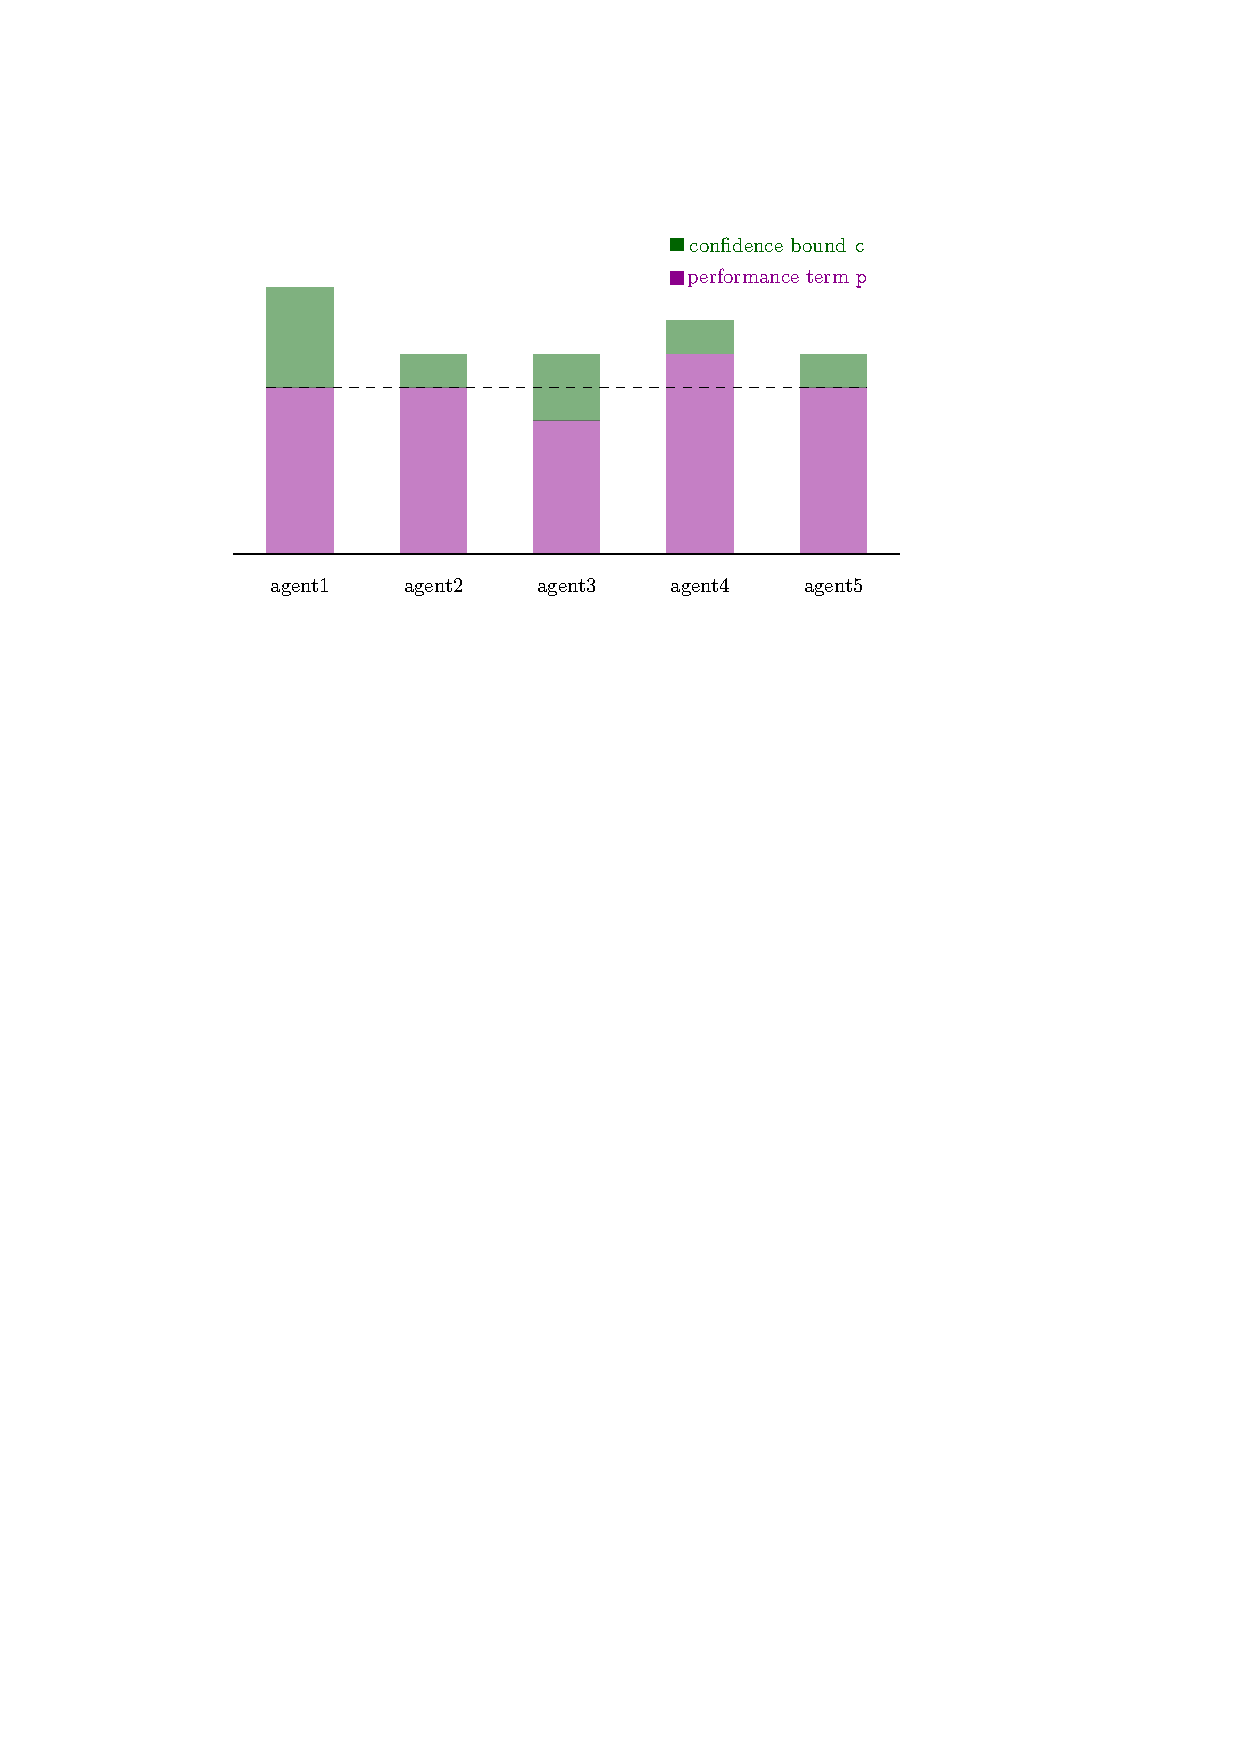
\includegraphics[scale=1, page=1]{ucb_demo.pdf}}
    \captionsetup{justification=centering}
    \caption{An example of UCB for 5 agents}
    \label{fig:UCB_example}
\end{figure}

\paragraph*{}
The process described above is done for every domain, since each domain is treated as its own, separate environment. Since a different instance of TheNegotiator takes part in each negotiation session, the UCB arrays have to be stored on disk. A subdirectory inside the given agent storage was used for that purpose, with a file for each combination of domain and preference profile (e.g. \texttt{domain07\_A.ucb} and  \texttt{domain07\_B.ucb} would both correspond to domain 7, but the first one would be for when we are given profile A and the second for when we are given B).

\paragraph*{}
Mathematically, the logic above is expressed like this:
\begin{equation} \label{eq:UCB}
    {ucb_{a}}' \quad = \quad \underbrace{\frac{[ucb_{a} \cdot (n_{a}-1)]+u}{n_{a}}}_{\texttt{p[a]}} \quad + \quad \underbrace{\sqrt{\frac{2 \ln N}{n_{a}}}}_{\texttt{c[a]}},
\end{equation}
\vspace{-0.5cm}		% brings the table a bit closer to the equation
\renewcommand{\arraystretch}{1} % Adjust the value as needed
\begin{longtable}{l l l}
    where 	& ${ucb_{a}}'$	& is the updated value of \texttt{ucb[a]} after picking it in the last round, \\
            & $ucb_{a}$  	& is the previous value of \texttt{ucb[a]}, \\
            & $n_{a}$ 		& is the number of times \texttt{a} has been picked, \\
            & $u$ 			& is the utility achieved in the last round by \texttt{a}, and \\
            & $N$ 		& is the number of total rounds played. \\
\end{longtable}

\paragraph*{}
The reader might also notice a problem with the UCB formula in equation \ref{eq:UCB}: on initialization, since $n_{a}=0$ for every agent $a$, all values in the UCB array will blow up to infinity. This is in fact intentional, as it forces the agent to play as every agent at least once, thus obtaining a an actual result from it in order to enhance/correct the neural network's prediction.
